% !TEX TS-program = pdflatex
% !TEX encoding = UTF-8 Unicode

% This is a simple template for a LaTeX document using the "article" class.
% See "book", "report", "letter" for other types of document.

\documentclass[11pt]{article} % use larger type; default would be 10pt

\usepackage[utf8]{inputenc} % set input encoding (not needed with XeLaTeX)

%%% Examples of Article customizations
% These packages are optional, depending whether you want the features they provide.
% See the LaTeX Companion or other references for full information.

%%% PAGE DIMENSIONS
\usepackage{geometry} % to change the page dimensions
% \geometry{a4paper} % or letterpaper (US) or a5paper or....
% \geometry{margin=1in} % for example, change the margins to 2 inches all round
 \geometry{
 a4paper,
 total={180mm,267mm},
 left=15mm,
 top=15mm,
 }

% \geometry{landscape} % set up the page for landscape
%   read geometry.pdf for detailed page layout information

\usepackage{graphicx} % support the \includegraphics command and options

% \usepackage[parfill]{parskip} % Activate to begin paragraphs with an empty line rather than an indent

%%% PACKAGES
\usepackage{booktabs} % for much better looking tables
\usepackage{array} % for better arrays (eg matrices) in maths
\usepackage{paralist} % very flexible & customisable lists (eg. enumerate/itemize, etc.)
\usepackage{verbatim} % adds environment for commenting out blocks of text & for better verbatim
\usepackage{subfig} % make it possible to include more than one captioned figure/table in a single float
% These packages are all incorporated in the memoir class to one degree or another...

%%% HEADERS & FOOTERS
\usepackage{fancyhdr} % This should be set AFTER setting up the page geometry
\pagestyle{fancy} % options: empty , plain , fancy
\renewcommand{\headrulewidth}{0pt} % customise the layout...
\lhead{}\chead{}\rhead{}
\lfoot{}\cfoot{\thepage}\rfoot{}

%%% SECTION TITLE APPEARANCE
\usepackage{sectsty}
\allsectionsfont{\sffamily\mdseries\upshape} % (See the fntguide.pdf for font help)
% (This matches ConTeXt defaults)

%%% ToC (table of contents) APPEARANCE
\usepackage[nottoc,notlof,notlot]{tocbibind} % Put the bibliography in the ToC
\usepackage[titles,subfigure]{tocloft} % Alter the style of the Table of Contents
\renewcommand{\cftsecfont}{\rmfamily\mdseries\upshape}
\renewcommand{\cftsecpagefont}{\rmfamily\mdseries\upshape} % No bold!

%%% END Article customizations
\usepackage{amsmath}
\usepackage{hyperref}
\usepackage{float}  
\usepackage{multirow}


%%% The "real" document content comes below...



\title{Starbucks capstone project}
\author{Thomas Heinemann}
%\date{} % Activate to display a given date or no date (if empty),
         % otherwise the current date is printed 

\begin{document}
\maketitle

\section{Project overview}

This is a recommendation engine project proposed by Starbucks to find out which demographic groups of customers respond best to certain types of offers. The underlying datasets include transactional and customer data, as well as information about the types of offers sent. The full set
of files, including the main Jupyter file with the detailed task, can be found at \cite{a}.
In addition, an approach for a simpler version of such a problem can be found here \cite{b}.
%\cite[1]{rfewf}


\begin{thebibliography}{2}

\bibitem{a} All project files: {\scriptsize \url{https://github.com/thomasheinemann/starbucks_promotion_type_exercise/}}

\bibitem{b} Simpler version of this project: {\scriptsize\url{https://github.com/thomasheinemann/starbucks_promotion_exercise/}}



\end{thebibliography}

\section{Introduction}
To begin with we first present the original introduction and task:


\begin{quote}
\begin{em}
This data set contains simulated data that mimics customer behavior on the Starbucks rewards mobile app. Once every few days, Starbucks sends out an offer to users of the mobile app. An offer can be merely an advertisement for a drink or an actual offer such as a discount or BOGO (buy one get one free). Some users might not receive any offer during certain weeks. 

Not all users receive the same offer, and that is the challenge to solve with this data set.

Your task is to combine transaction, demographic and offer data to determine which demographic groups respond best to which offer type. This data set is a simplified version of the real Starbucks app because the underlying simulator only has one product whereas Starbucks actually sells dozens of products.

Every offer has a validity period before the offer expires. As an example, a BOGO offer might be valid for only 5 days. You'll see in the data set that informational offers have a validity period even though these ads are merely providing information about a product; for example, if an informational offer has 7 days of validity, you can assume the customer is feeling the influence of the offer for 7 days after receiving the advertisement.

You'll be given transactional data showing user purchases made on the app including the timestamp of purchase and the amount of money spent on a purchase. This transactional data also has a record for each offer that a user receives as well as a record for when a user actually views the offer. There are also records for when a user completes an offer. 

Keep in mind as well that someone using the app might make a purchase through the app without having received an offer or seen an offer.
\end{em}
\end{quote}

So how do we proceed?
A simple statistical evaluation based on the frequency of offer completions or views per customer may not work, as we do not have huge data sets for each person with and without receiving, viewing and completing a considered offer type. Also, a customer being researched may not have exactly the same profile as those provided.
We therefore improve the statistics by reducing the value set of the customer profile data.
However, this is not enough, so we train models to predict as accurately as possible whether the customer is worth promoting or not.
The advantage of this is that these models also make good use of information from other more or less closed customer profiles.

In the following sections, we provide definitions, present the modelling approach, summarise the results for each type of offer and conclude with our main findings in the conclusion section.


\section{Definitions}
\textbf{Main offer types to be considered:}
\begin{itemize}
\item BOGO (buy one get one free) offer: If the customer buys the praised product of this offer then this person gets the same product on top for free.
\item discount offer: If the customer spends a certain amount then this person receives a discount.
\item informational offer: These offers just show the customer an advertisement for a product, e.g., a drink. In the given data, however, there is no offer completion record.
\end{itemize}
\noindent\textbf{Offer instance:} 
An offer sent for one specific customer, at one specific time (offer\_received\_time). So each offer instance is addressed with the key \textbf{[offer\_id, person, offer\_received\_time]} which is found being unique.
\\
\\
\noindent\textbf{Offer events:} 
\begin{itemize}
\item offer received
\item offer viewed (can also happen after offer is completed or no longer valid)
\item transaction = the customer makes a transaction of a certain amount 
\item offer completed = the difficulty challenged by the offer has been overcome with the current transaction
\end{itemize}
\noindent\textbf{Offer event times:} 
Times of the offer events above are further denoted as "offer\_received\_time", "offer\_viewed\_time", "transaction\_time", and "offer\_completed\_time".
\\
\\
\textbf{Offer event record (OER): } An OER consists of the offer receiving event, a possible offer viewing event as well as an offer completed event, and all transaction events belonging to one specific offer instance.
Accordingly like each offer instance, each OER is addressed with the unique key [offer\_id, person, offer\_received\_time].
For each person we also define one OER related to no-offer times.
These are addressed as [offer\_id="no offer", person, offer\_received\_time=0].
Each OER has an offer validation interval starting at its offer\_received\_time and finishes with the $$\mathrm{offer\_time\_out}=\mathrm{offer\_received\_time}+24 \times \mathrm{duration}.$$ 
The duration marks the maximum offer-specific time interval in days, in which the offer can be valid, if not completed earlier.
\\
\\
\textbf{States of an offer instance}: 
\\
Each offer instance is characterized by the binary state variables "promoted", "viewed" and "completed".
Their calculation requires the corresponding OER and is shown in the following table.
\\
\\
\begin{tabular}{|c||c|c|c|c|}
 \hline
state variables of an offer instance & calculation in terms of logical expressions \\ 
\hline
\hline
promoted & offer\_id $\ne$ "no offer"\\ 
\hline
\multirow{ 2}{*}{viewed} &  $\mathrm{offer\_viewed\_time} \le \mathrm{offer\_end\_time}$\\ 
&  with: $ \mathrm{offer\_end\_time}=Min(\mathrm{offer\_time\_out},\mathrm{ offer\_completed\_time})$\\ 
\hline
completed & $\mathrm{ offer\_completed\_time} \le \mathrm{offer\_time\_out} $ \\ 
\hline
\end{tabular}
\\
\\
\\
\textbf{Consumption during offer:}
It is a quantity referring to one OER.
It is defined as the sum of all transactions done in an OER where each transaction lies in the time interval [offer\_received\_time, offer\_time\_out].


\section{Modeling approach}
\subsection{Data flow}
The data flow along our prediction pipeline starts with the original customer profile attributes and finishes with a decision on whether to promote that person or not. The first step consists in cleaning NaN values and introducing categorical variables for the gender attribute. In the second step, model 1 predicts an early viewing preference used to sort out "lazy viewers".  For predicting the final promotion decision, we used in step 3 the model 2 which is specifically fitted for the each offer type separately.
\begin{figure}[H]
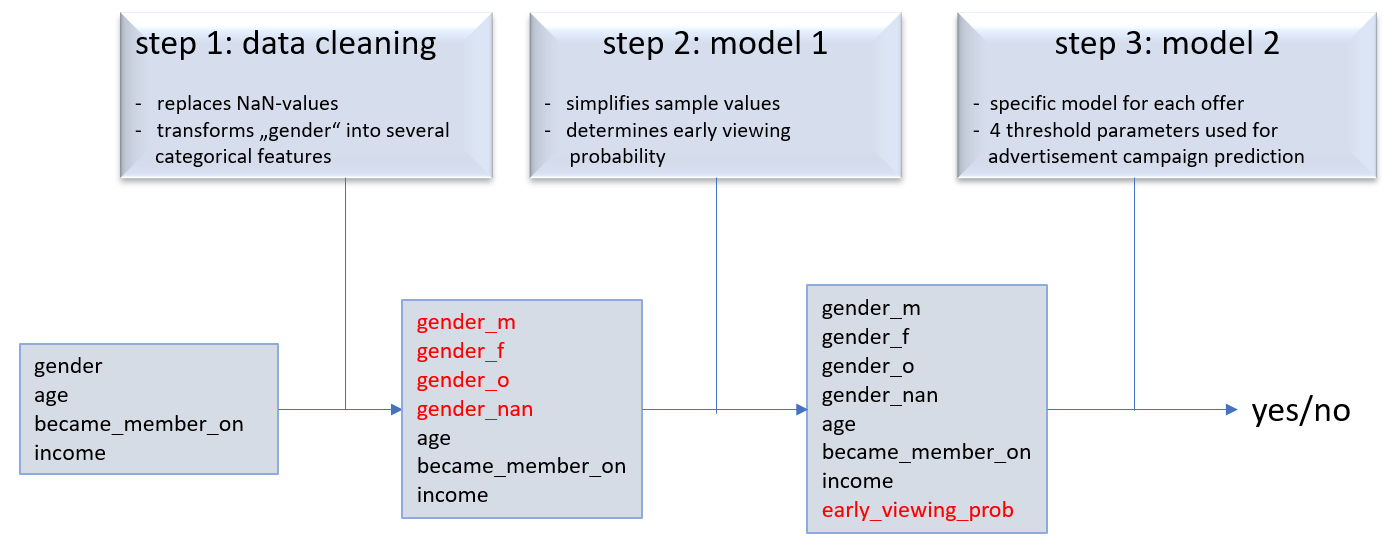
\includegraphics[width=0.95\textwidth]{dataflow.png}
\caption{Data flow showing a prediction  pipeline for customer profile attributes  "gender", "age", "became\_member\_on", "income" towards a "yes/no"-prediction for an advertisement campaign. For each offer type a differently fitted version of model 2 is used. The models 1 and 2 have been fitted using customer profile attributes and the customers' offer event records (OERs).}
\end{figure}

\subsection{Step 1: data preparation}
The customer profile data is first undergoing a NaN-value treatmet for the income.
In particular, customers who do not provide an income, are remarked as having an income of -10 k dollar.
Another issue being treated within this step is the gender attribute which is categorical without order and thus splitted into one-hot-encoded attributes for each class label yielding "gender\_m", "gender\_f", "gender\_o",  and "gender\_nan" (denotes if no gender is provided).




\subsection{Step 2: model 1}
Model 1 has the task of simplifying the value sets of the customers' integer features "age", "become\_member\_on" and "income" using a transformer to achieve 10-year-steps for the "age", 1-year steps for "become\_member\_on" and 10 k dollar steps for "income".
Then, in a second transforming process,  a test-set customer yields, within the framework of model 1, a viewing preference encoded in the attribute, "early\_viewing\_prob" (probability for the offer to be viewed within 48 h).
The underlying model of the second transformer is fitted with all the cleaned customer profile data of the profile training set along with informations of their offer instances' states. The offer instances to be considered comprise only the customers' non-overlaping  ones. This constraint was chosen because multi-offer effects may be quite complex and would constitute a further investigation step probably requiring more data.


%\begin{figure}[H]
%\begin{center}
%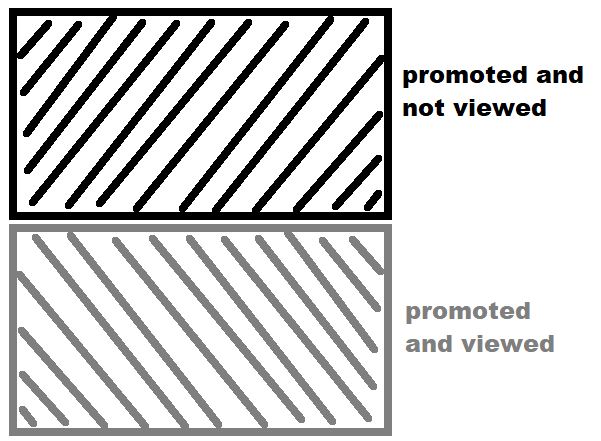
\includegraphics[width=0.4\textwidth]{venn_diagram.png}
%\caption{\label{fig:venn1}Venn diagram visualizing the task of model 1 which has to perform a prediction whether a customer is one who views an offer or one who does not. }
%\end{center}
%\end{figure}

\subsection{Step 3: model 2 (offer specific model)}

In this step, an offer specific model comes into play. Accordingly, for each offer type, a separate instance of this model is used.
The model itself makes use of cleaned customer profile data and all the customers' OERs of non-overlaping offer instances of the considered offer type and their no-offer OERs.
The "offer completion" states for the no-offer instances are calculated in this model as if the customer was promoted with the offer type considered in this model.
To be precisely, a difficulty had to be overcome that scales with the ratio between the no-offer and offer duration.

With respect to states of offer instances, we generally distinct six since an offer can be  sent or not, can be viewed (if promotion exists) or not, and completed or not.
A grouping of these six classifications into four different labels forms the base of the current model and is shown in the following table.

\begin{center}
{\Large
\begin{tabular}{|c||c|c|c|c|}
 \hline
&\multicolumn{3}{c|}{  states of offer instances}\\
 label & promoted & viewed & completed \\ 
\hline
\hline
I & yes & yes & yes \\ 
\hline
\multirow{ 2}{*}{II} & no & no & yes \\ 
 & yes & no & yes \\ 
\hline
III & yes & yes & no \\ 
\hline
\multirow{ 2}{*}{IV} &no & no & no \\ 
 & yes & no & no \\ 
 \hline
\end{tabular}
}
\end{center}

The goal of model 2 ist to make use of the upper 4-label classification of ofer instance states to predict customers who complete the offer only if viewed.
These customers ideally have only offers with states labeled I and IV, respectively. In Fig. \ref{fig:venn2} a Venn diagram is shown that depicts ideal customer sets along with the one we are interested in. We hereby define an ideal customer as one for who the offer completion status solely depends on the viewing status or is even independent of the latter.
This definition leads to the four different types of ideal customers shown in the figure.
\begin{figure}[H]
\begin{center}
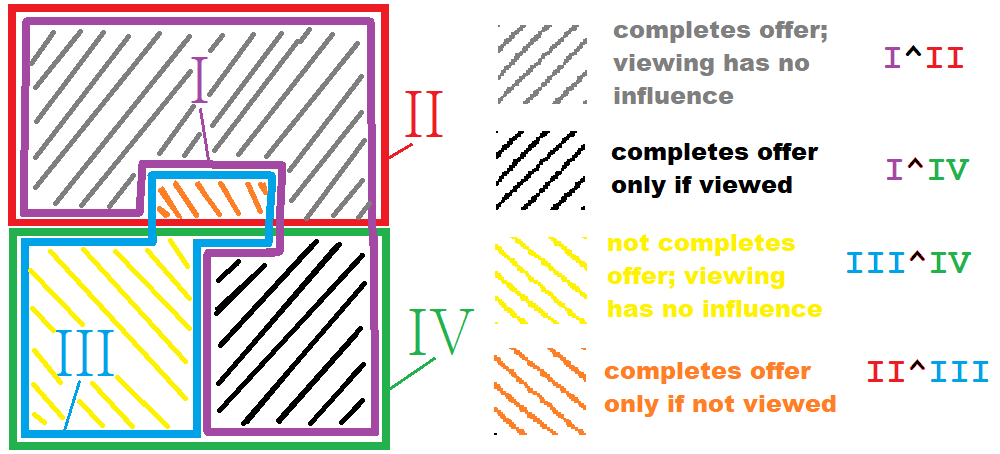
\includegraphics[width=0.7\textwidth]{venn_diagram2.png}
\caption{\label{fig:venn2}A Venn diagram representing a grouping of ideal customers into four disjunct sets filled with differently colored diagonal stripes is shown. In each set only two distinct offer instance state labels occure (represented by Roman numbers). 
%  Model 2 is designed to predict people who "complete an offer only if viewed" (black striped area).
}
\end{center}
\end{figure}
Unfortunately, our customers are not ideal, so each customer behaves differently with respect to each singular offer instance.
We can therefore only predict what behavior the customer is most likely to reveal by assuming a correlation between the customer's profile and their offer instances' states.

In order to determine whether a customer is "completing the offer only if viewed", we create one predictor to distinguish between customer profiles having states with label II vs. those having states with label IV and in analogy a second one to distinguish between I vs. III.
Using their prediction probabilities for customers with label I as well as label IV states, one can achieve a good estimate for the black-striped area. To do so, the threshold parameters named as $p_1$ and $ p_2$ for both predictors have to be overcome.

However, some customers even get repelled from buying when viewing an advertisement (see orange-striped area). These customers are not in the black-striped area but since the border areas are fuzzy we
further included a third predictor (with threshold parameter $p_3$) distinguishing customer sets with label I $\cup$ IV vs. II $\cup$ III. This allows a seperate tuning of the border between the orange and black-striped area as well as the border between the orange and gray-striped area. In addition, we implemented a fourth threshold parameter $p_4$ for the early viewing probability as determined in model 1, for sorting out lazy viewers in the results set.
This may prevent having to much customers being unknowingly rewarded.

The threshold parameters are optimized for each model using a 3-fold cross validation method.
The scoring metric for the validation sets  as well as the test set, used for each model 2, is defined in the following.
\subsection{Scoring metric}
The scoring metric was chosen to take two important aspects into account.
On the one hand we want to maximize the number of customers who complete an offer when receiving it. The underlying metrics to maximize is the "incremental response rate" ("irr").
On the other hand, we aim at having a gain in consumption by maximizing a shifted version of the "net incremental reveniew" ("nir").
This prevents our recommendation algorithm to promote too many customers whose reward makes them spend less as they are too satisfied.
As a scoring  metrics we accordingly used a compromise being a product of both former metrics, i.e.
\begin{align}
\text{scoring metric}= irr \times nir
\end{align}
Both metrics are defined in the following.
%
\\
\\
\text{\bf Incremental response rate "irr" (for offer type X):}
\begin{align}
irr=\frac{ n_{prom,compl} }{ n_{prom}} &-\frac{ n_{no\ prom,compl} }{ n_{no\ prom}}
\\
\nonumber\\
n_{prom,compl}:& \text{number of instances of offer type X which are completed}\nonumber
\\
n_{prom}:& \text{number of instances of offer type X}\nonumber
\\
n_{no\ prom,compl}:& \text{number of no-offer instances whose consumption rate would have completed}\nonumber
\\
& \text{an offer of offer type X}\nonumber
\\
n_{no\ prom}:& \text{number of no-offer instances}\nonumber
\end{align}
\text{\bf Shifted net incremental  revenew  "nir" (for offer type X):}
We take the sum of the consumptions of completed offers (of offer type X) minus the sum of consumptions of no-offer instances whose consumption rate would fulfill an offer completion event of offer type X.
Each consumption is normalized by its correspnding offer/no-offer duration.
\begin{align}
nir=& \sum_{\substack{i \in \text{ completed offer}\\ \text{instances in}\\ \text{ test set}}} \frac{ \text{consumption(i) }}{ \text{duration(i) }} -   \sum_{\substack{k \in \text{ "completed" } \\ \text{no-offer instances  }\\ \text{in test set}}} \frac{  \text{consumption(k) }}{ \text{ duration(k) }}-\text{shift}\cdot  n_{\text{test}}
\\
\nonumber\\
 \text{consumption }(x):& \text{\ consumption during offer/no-offer instance x}\nonumber\\ 
 \text{duration }(x):& \text{\ duration of offer/no-offer instance x}\nonumber\\ 
 n_{\text{test}}:& \text{\ number of all offer/no-offer instances (in the test set)}\nonumber\\ 
 n_{\text{train}}:& \text{\ number of all offer/no-offer instances (in the training set)}\nonumber\\ 
 \text{shift}=& {\tiny   \frac{1}{ n_{\text{training}}}   \left(
 \sum_{\substack{i \in \text{ "completed" offer}\\ \text{instances in}\\ \text{ training set}}} \frac{ \text{consumption(i) }}{ \text{duration(i) }} -   \sum_{\substack{k \in \text{ "completed" } \\ \text{no-offer instances  }\\ \text{in training set}}} \frac{  \text{consumption(k) }}{ \text{ duration(k) }}  \right)    }\nonumber
\end{align}




\section{Results}



\subsection{Diagram for the test set}
We present in this susection a cluster analysis among all customers using five histograms covering gender, income, age, membership begin, and viewing preference and thereby stack the bin counts for each cluster on top of each other using different colors. The clusterization has been performed in a five dimensional space spanned by all the former-mentioned demographic attributes represented by one histogram each.
The optimal number of clusters have been detected using the kmeans++ algorithm with the help of the silhoutte score and is limited hereby to five for simplicity.


\begin{figure}[H]
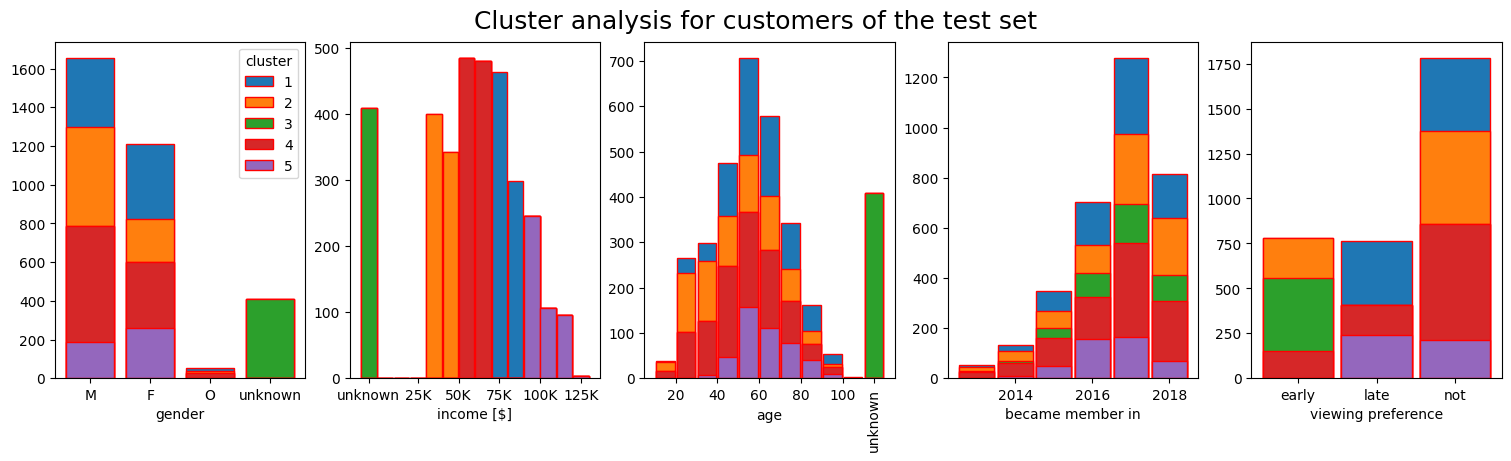
\includegraphics[width=1\textwidth]{results/results_test_set.png}
\caption{Cluster anaylis for all customers in the test set using 5 clusters. With respect to the clusterization, we can recognize that people, who do not provide information about gender, income and age are entirely early viewers. 
Customers earning more than 70 k are slightly dominated by women. Those earning more than 90 k dollar are not under 40 years old and do not tend to view offers within two days.}
\end{figure}

\subsection{Diagrams with observations for each offer type}
In this subsection, we briefly analyze for each offer type the customers we recommend for a promotion and also those we do not want to recommend according to the here presented strategy.
Each figure represents the results of one offer type analysis and consists of three rows of diagrams which cover the demographic information gender, income, age, membership begin, and viewing prefererence.
The upper row of diagrams displays data of all customers and highlights the customers who should be promoted according to the found strategy.
The mid row comprises only data of customers to be promoted, whereas the bottom row covers only customers not to be promoted.
The customers' demographic data in the corresponding histograms have been clustered in the five dimensional space spanned by all the former-mentioned demographic attributes. The clusterization has been performed separately for the  target and not-to-target customers.
\subsubsection{Diagrams for "bogo" offers}

\begin{figure}[H]
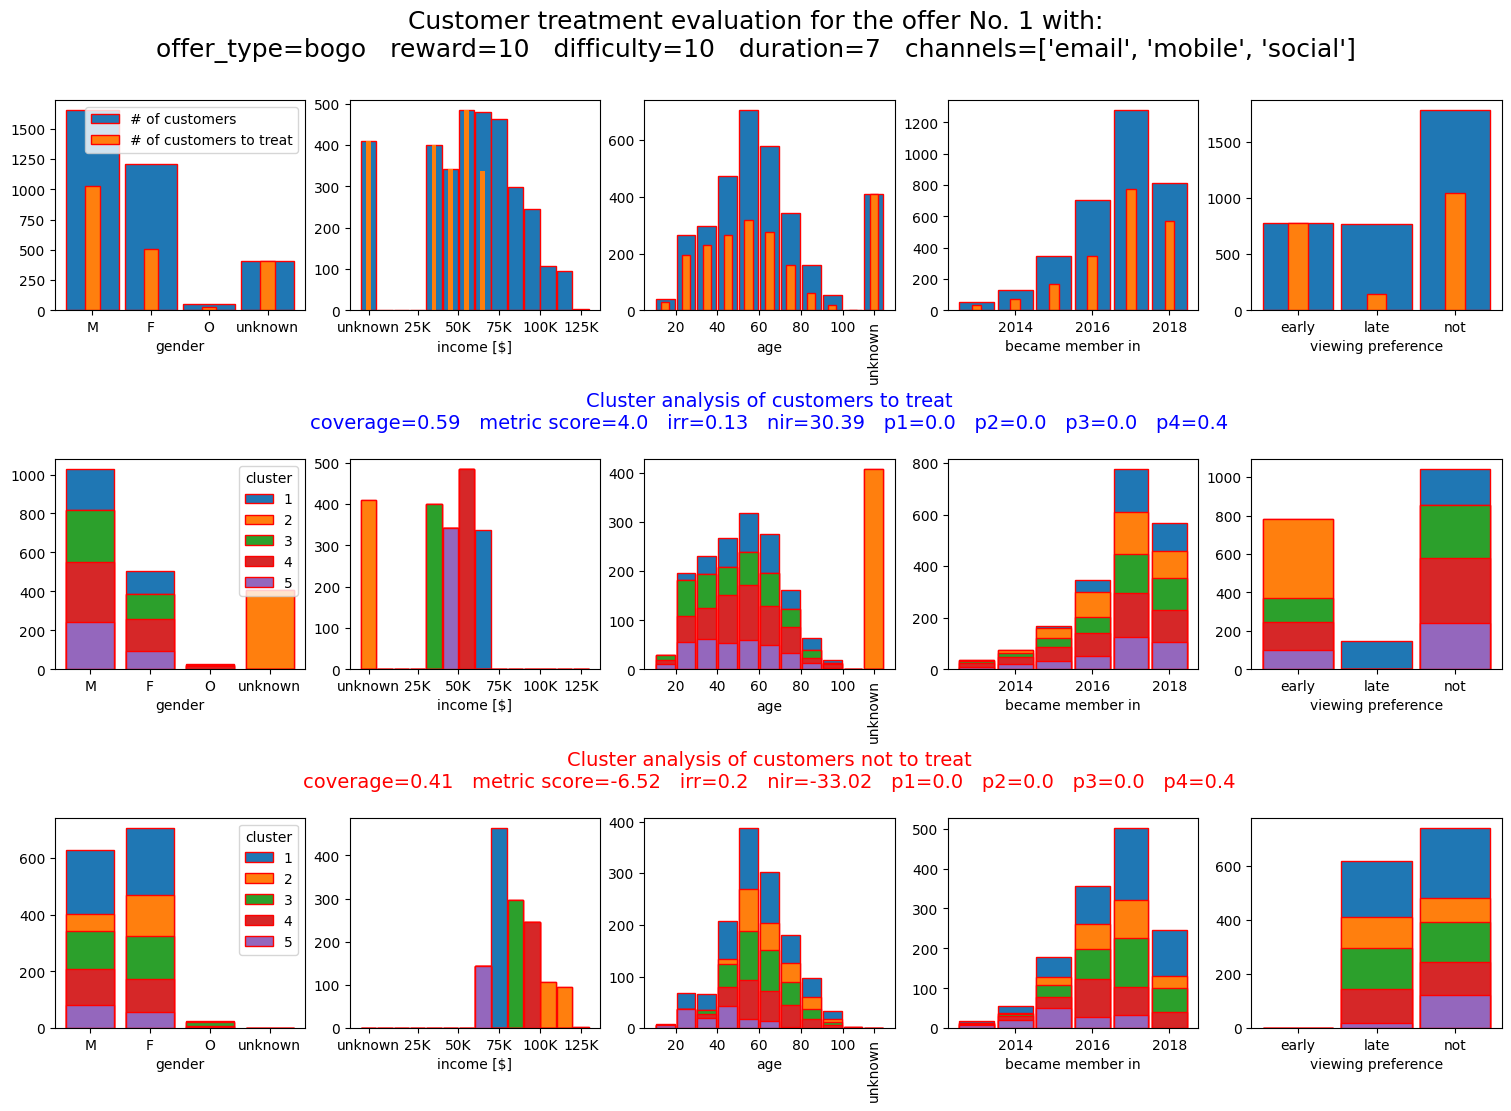
\includegraphics[height=0.5\textheight]{results/results1.png}
\caption{Customers with  incomes up to 70 k dollars are worth being addressed by this offer. Those who do not provide demographic information should be included as well. The considered customers tend to view early or rather not. }
\end{figure}
\begin{figure}[H]
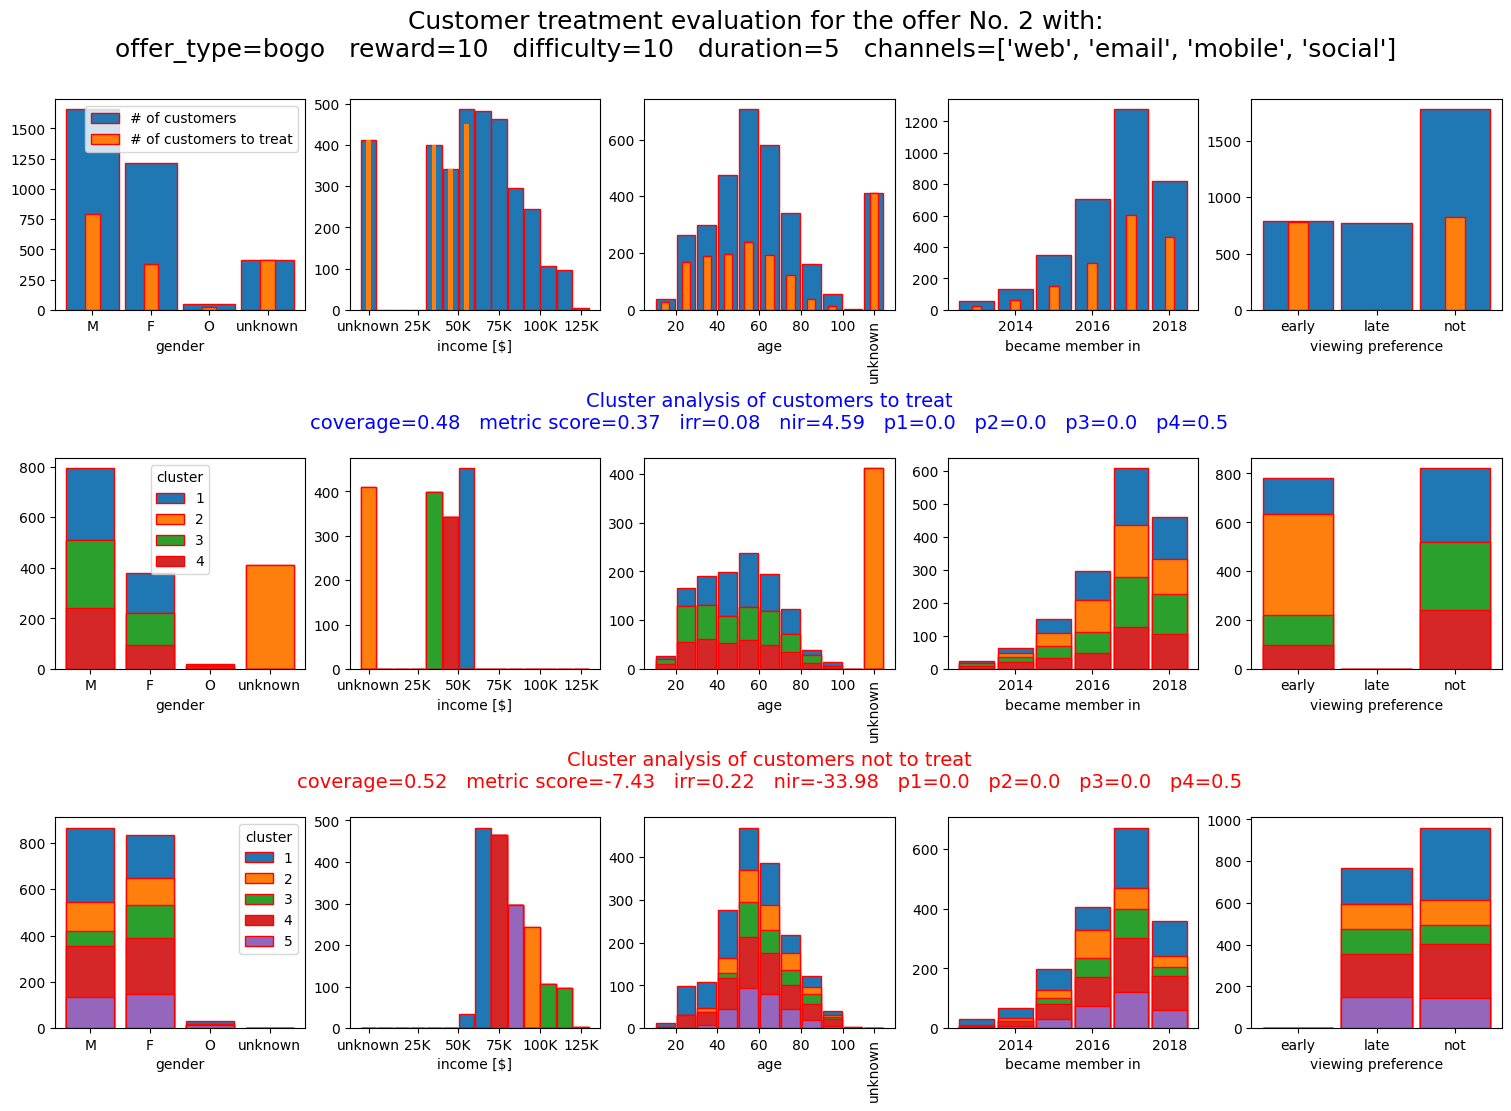
\includegraphics[height=0.5\textheight]{results/results2.png}
\caption{Customers with  incomes up to 60 k dollars are worth being addressed by this offer. Those who do not provide demographic information should be included as well.}
\end{figure}
\begin{figure}[H]
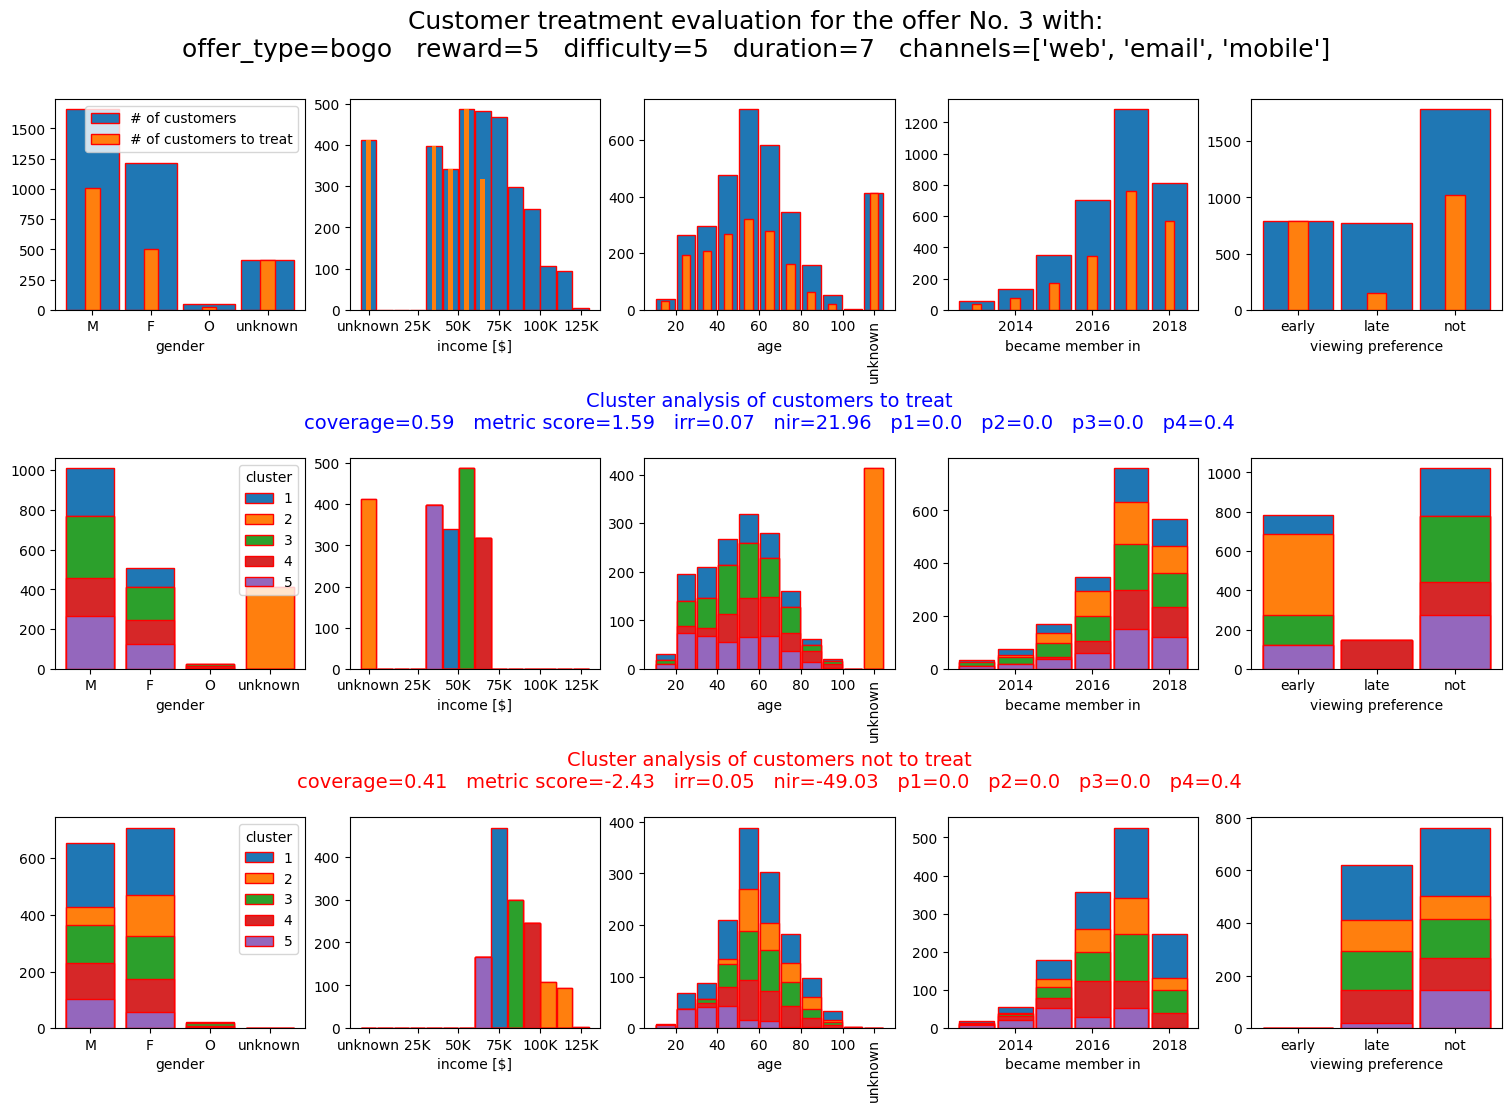
\includegraphics[height=0.5\textheight]{results/results3.png}
\caption{Customers with  incomes up to 70 k dollars are worth being addressed by this offer. Those who do not provide demographic information should be included as well. }
\end{figure}
\begin{figure}[H]
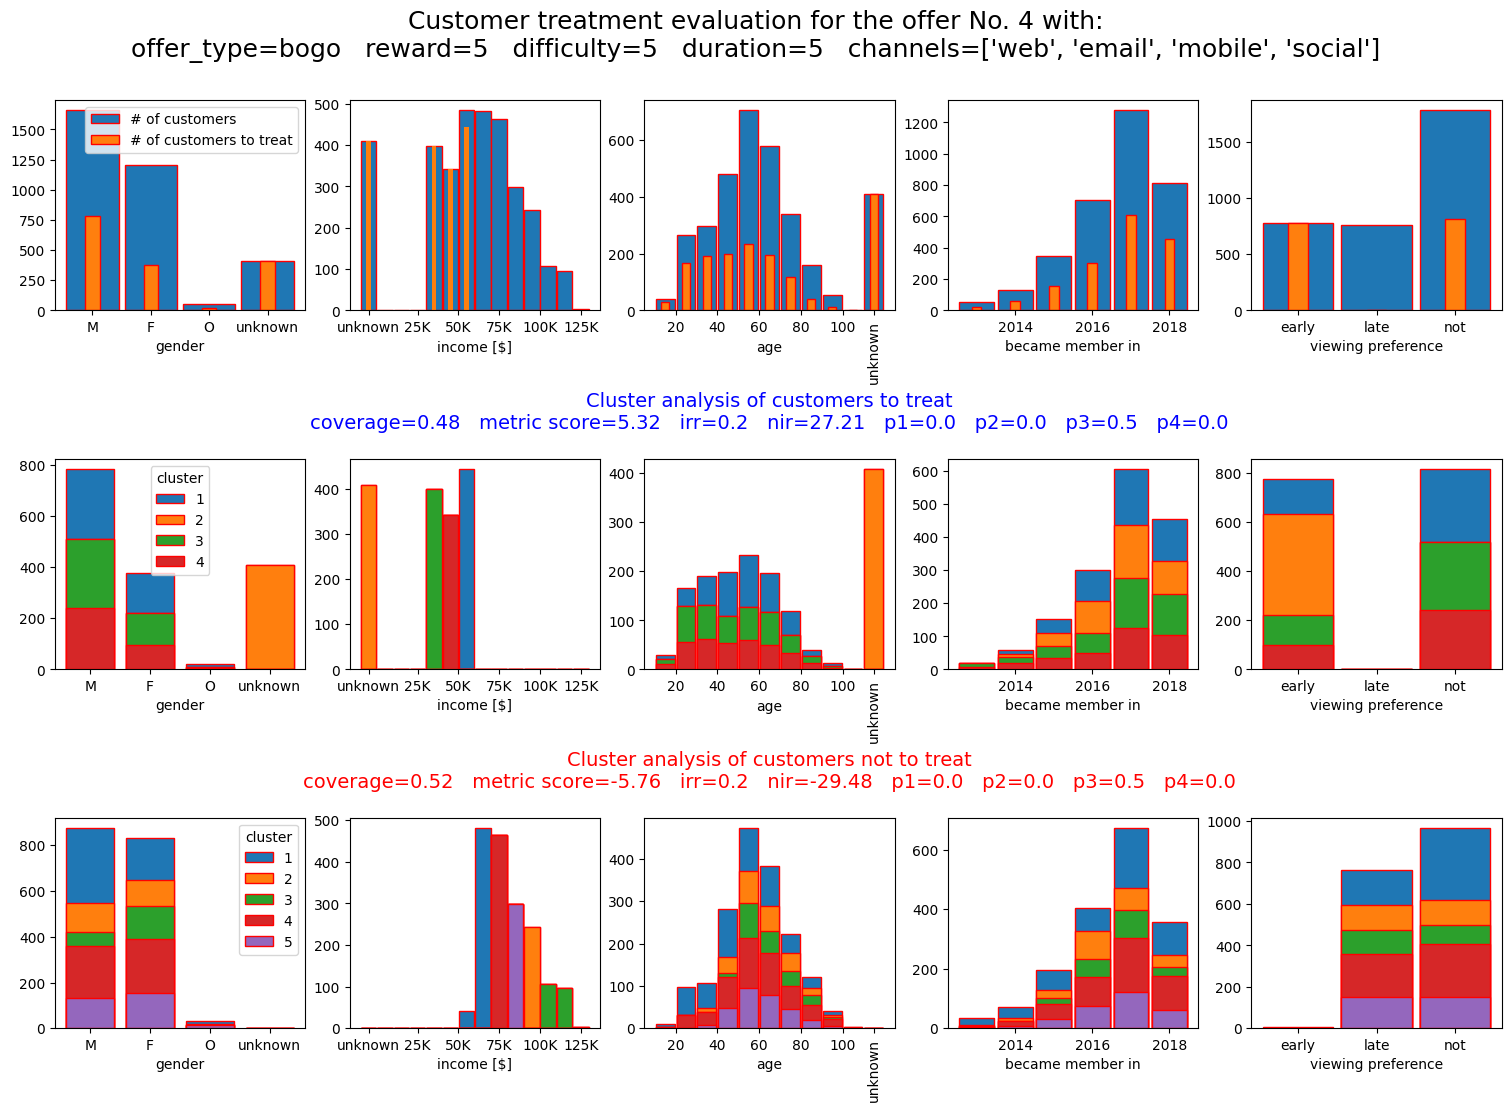
\includegraphics[height=0.5\textheight]{results/results4.png}
\caption{Customers with  incomes up to 60 k dollars are worth being addressed by this offer. Those who do not provide demographic information should be included as well. }
\end{figure}
\subsubsection{Diagrams for "discount" offers}

\begin{figure}[H]
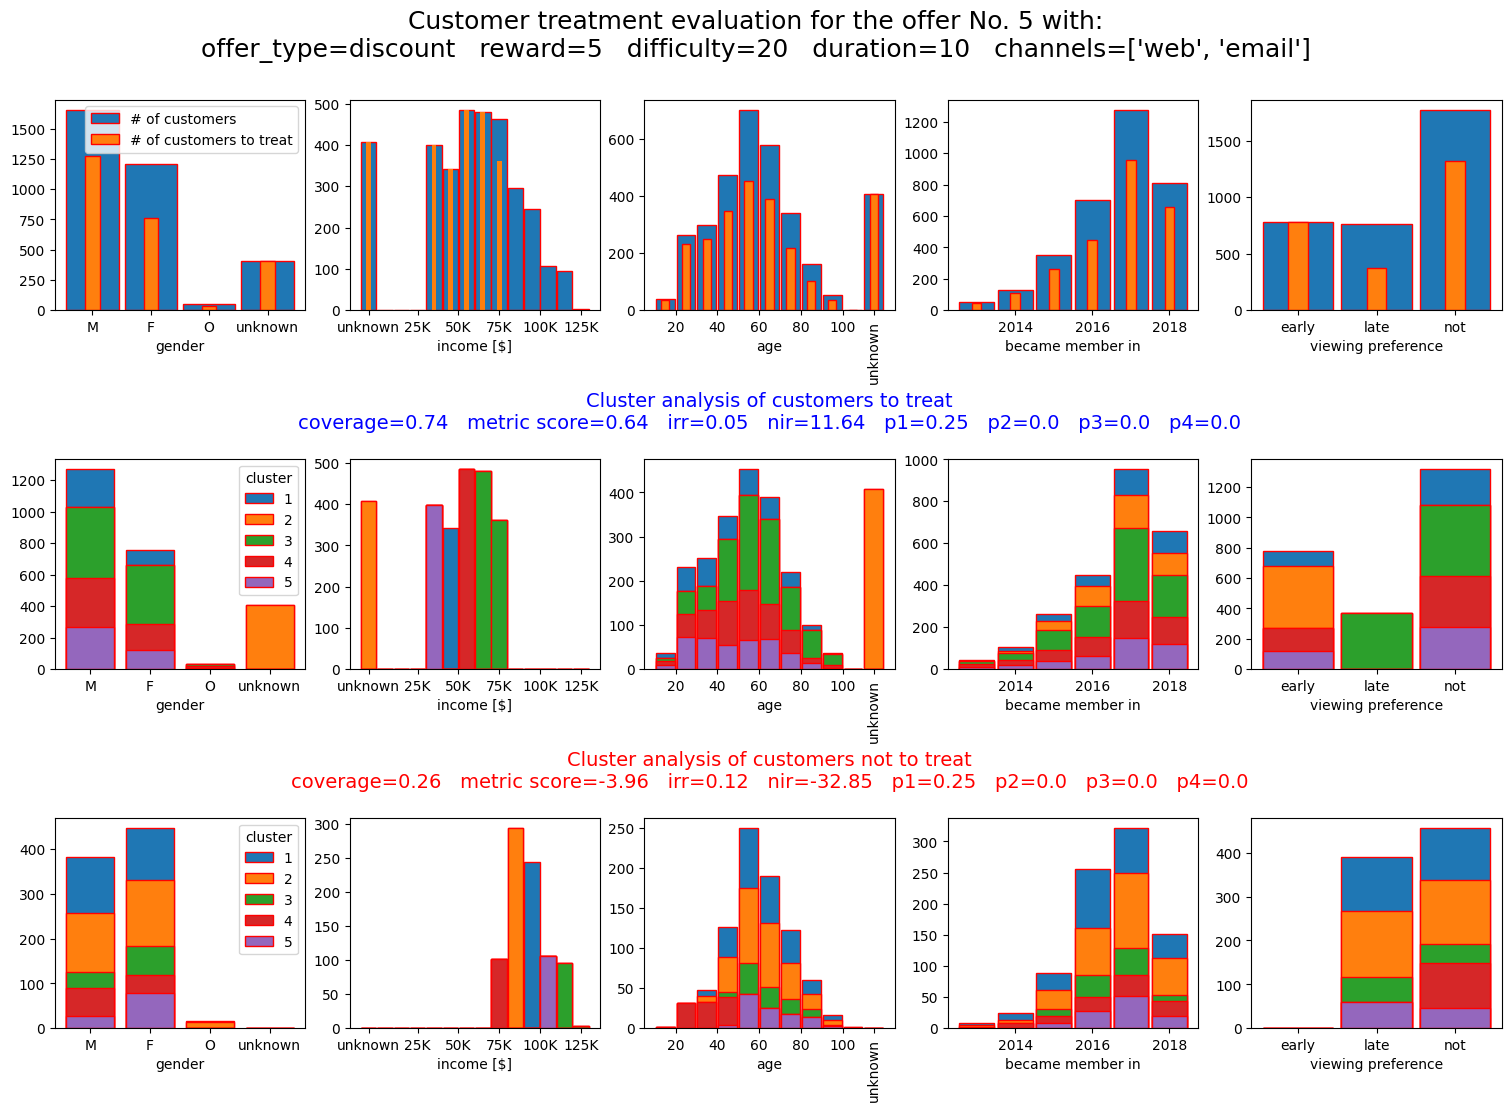
\includegraphics[height=0.5\textheight]{results/results5.png}
\caption{Customers with  incomes up to 80 k dollars are worth being addressed by this offer. Those who do not provide demographic information should be included as well.}
\end{figure}
\begin{figure}[H]
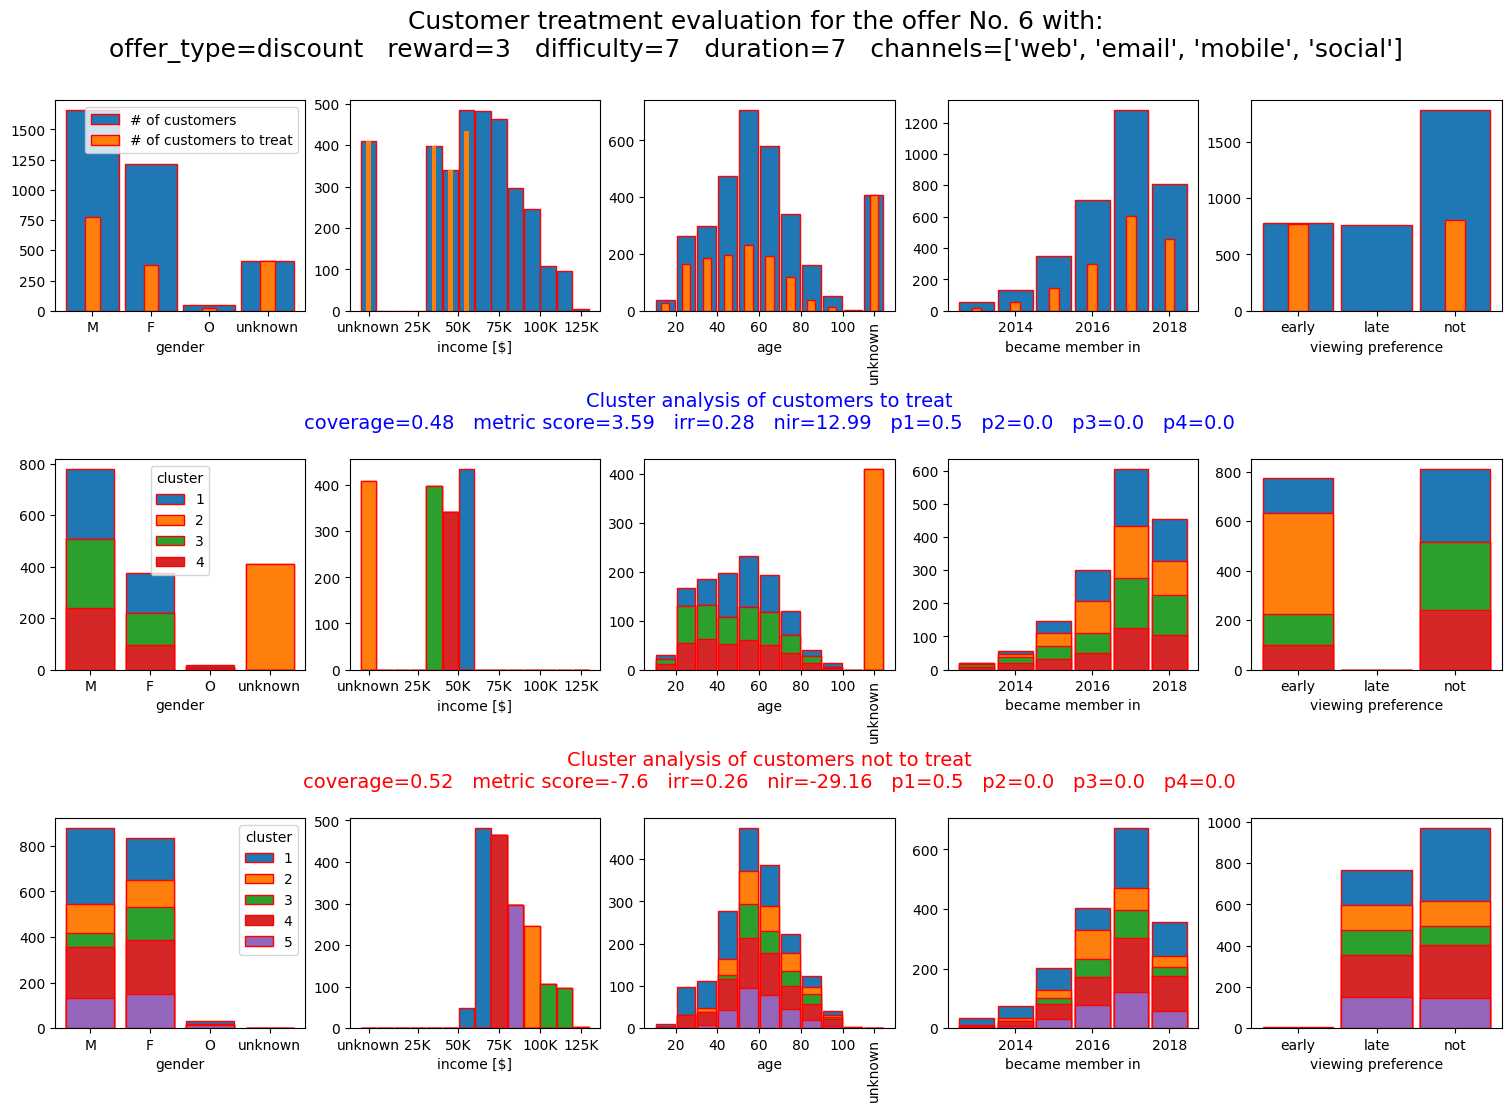
\includegraphics[height=0.5\textheight]{results/results6.png}
\caption{Customers with  incomes up to 60 k dollars are worth being addressed by this offer. Those who do not provide demographic information should be included as well.}
\end{figure}
\begin{figure}[H]
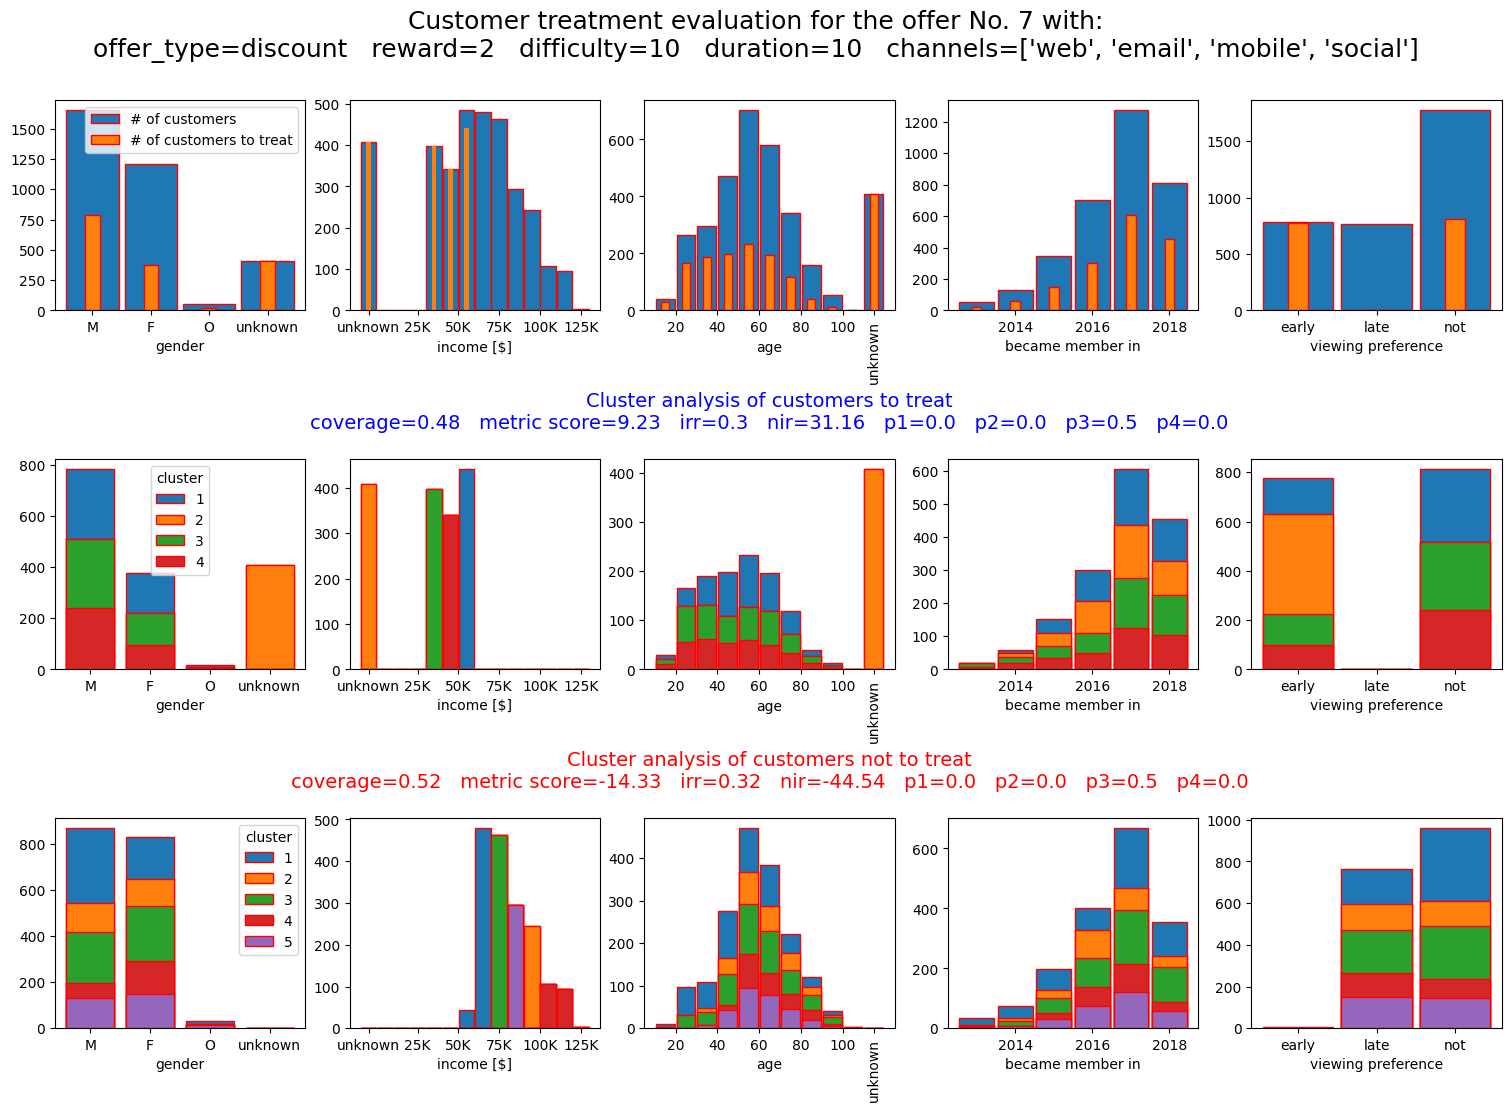
\includegraphics[height=0.5\textheight]{results/results7.png}
\caption{Customers to be addressed are basically the same as in offer type 6. Howeer, this offer type has a stronger value in the metric score.}
\end{figure}
\begin{figure}[H]
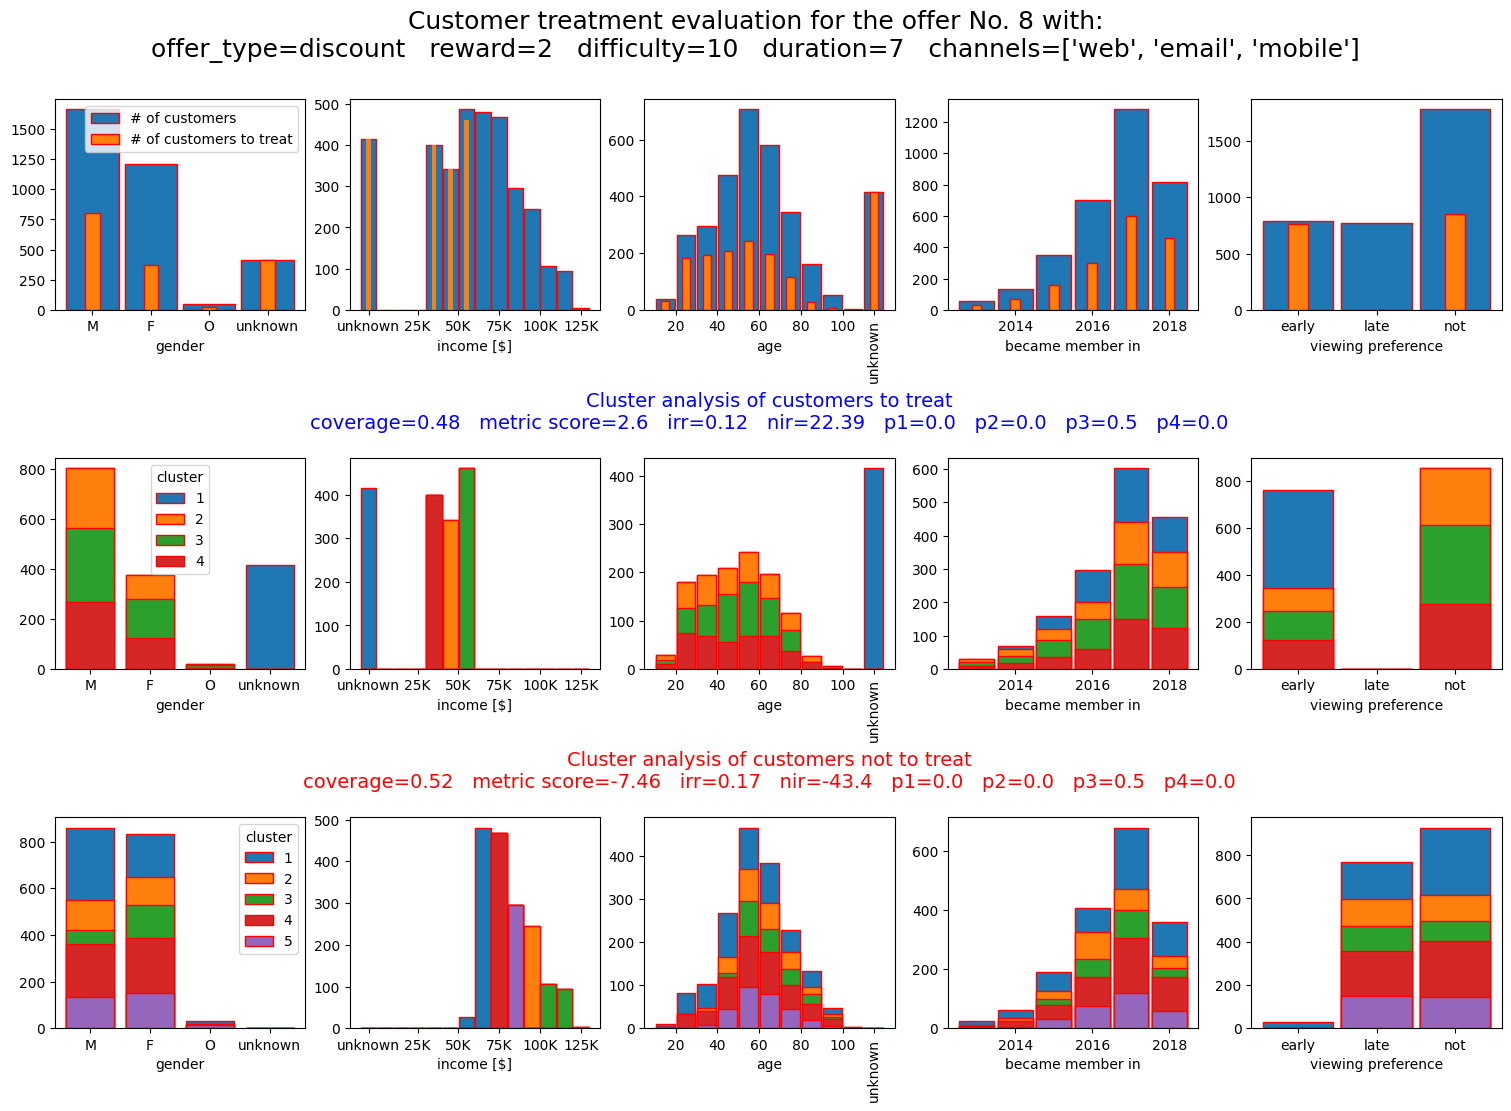
\includegraphics[height=0.5\textheight]{results/results8.png}
\caption{Customers to be addressed are basically the same as in offer type 6. Howeer, this offer type has a weak value in the scoring metric. }
\end{figure}
\subsubsection{Diagrams for "informational" offers}
\begin{figure}[H]
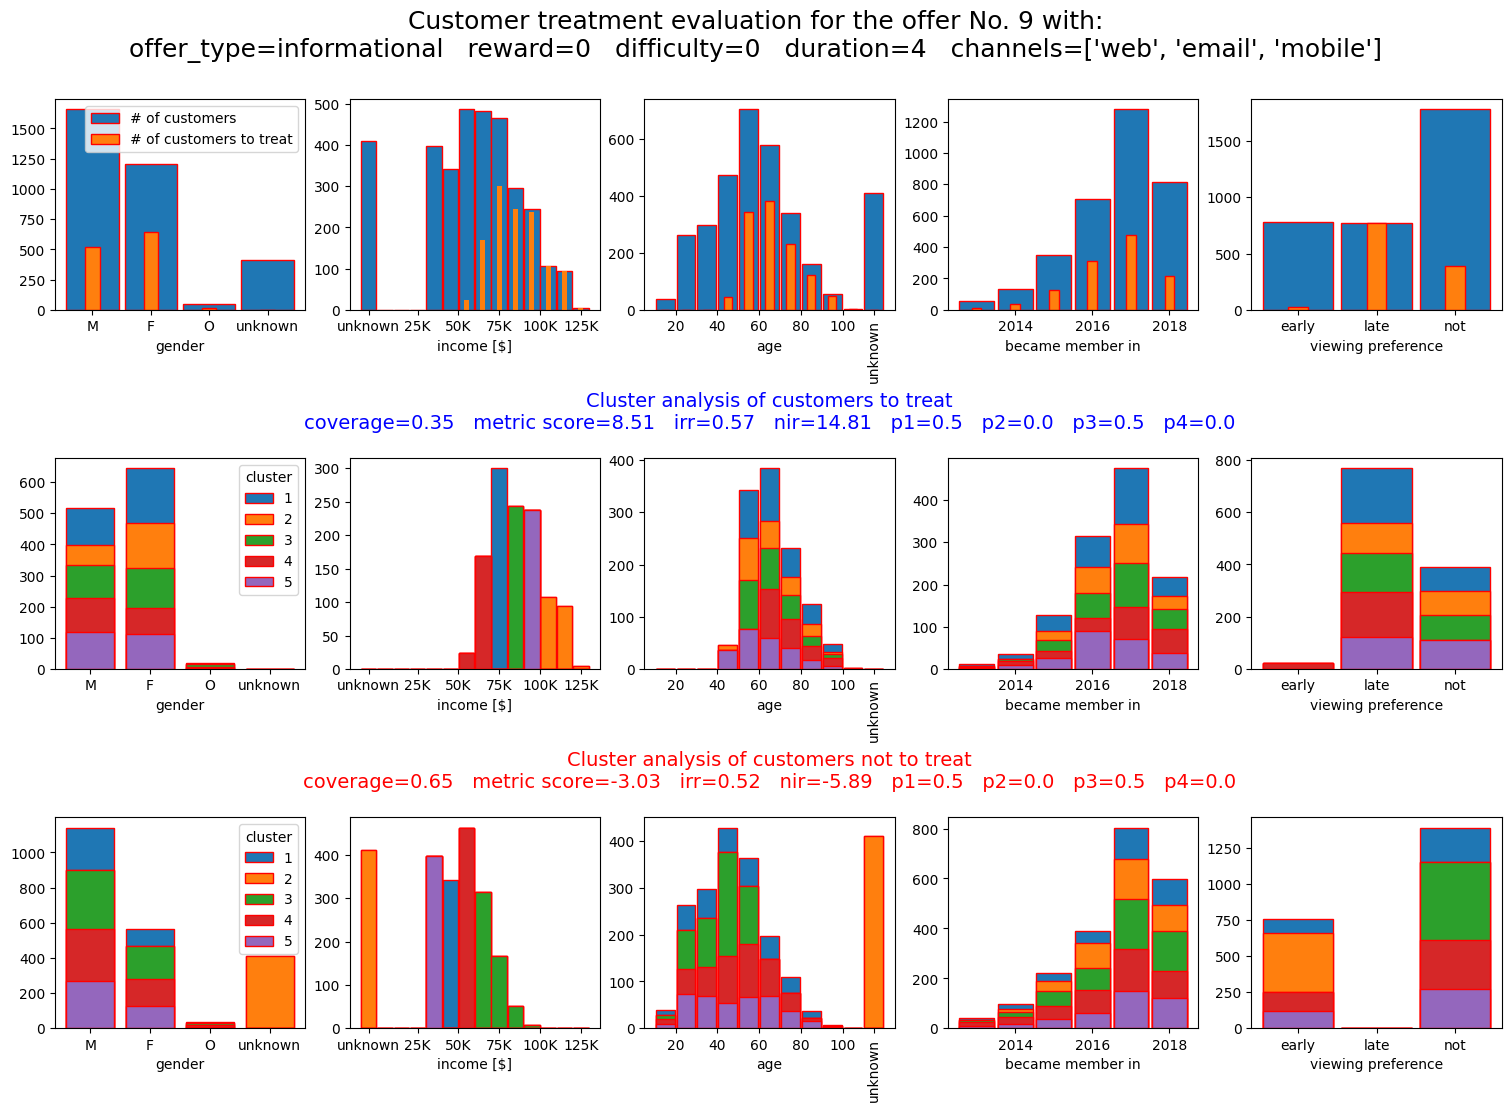
\includegraphics[height=0.5\textheight]{results/results9.png}
\caption{All customers earning at least 60 k dollars should be adressed by this offer. These customers tend to view lately or rather not. Customers not providing demographic information should be excluded.}
\end{figure}
\begin{figure}[H]
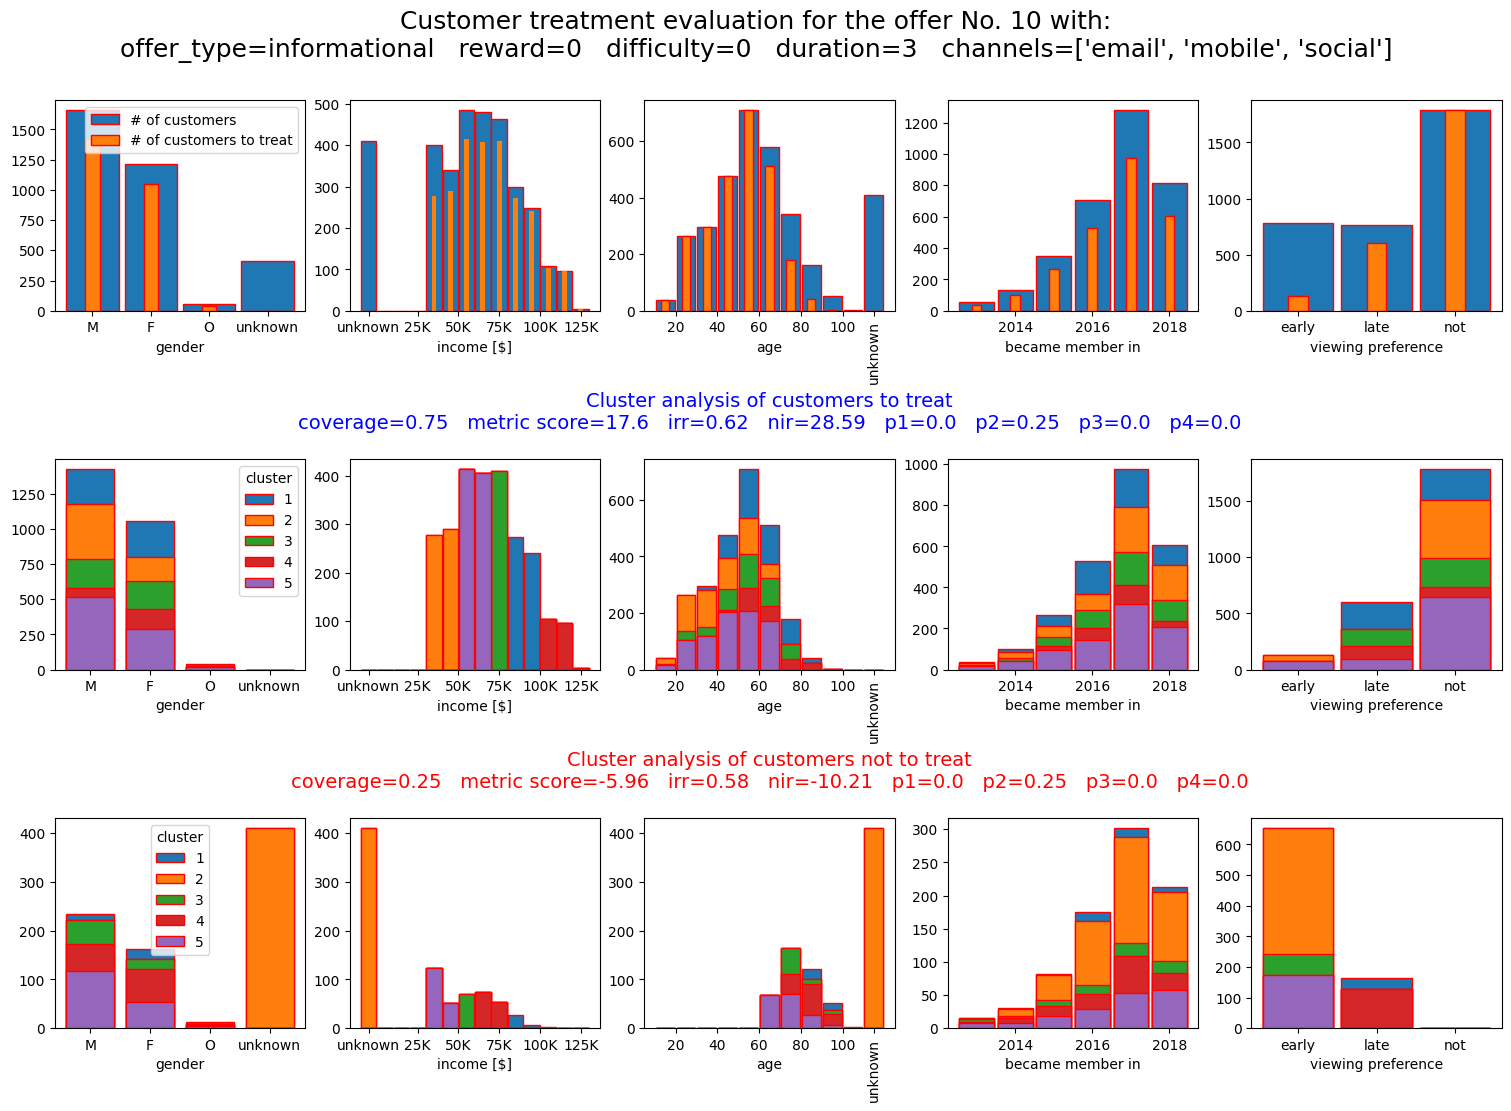
\includegraphics[height=0.5\textheight]{results/results10.png}
\caption{Primarily young and mid-aged customers are worth being addressed by this offer. These customers tend to view lately or rather not. Customers not providing demographic information should be excluded. From those earning 70 k dollars or less, only those who tend to view lately are within the target group.}
\end{figure}


\section{Conclusion}
BOGO and discount offers are primarily suitable for low and mid-income customers. The best BOGO offer is offer type No. 4 and designed for customers earning up to 60 k dollar.
It has a  5-day vailidity period and a 5 dollar difficulty to overcome. 
The best discount offer is offer type No. 7 possessing a 7-day vailidity period, a 10 dollar difficulty and a 2 dollar reward.
Also this offer type is designed for customers earning up to 60 k dollar but has a metric score being twice compared to the best BOGO one.
Nonetheless, both money-saving offers, BOGO and discount, seem not designed for customers in the higher income region.
With respect to the informational offers, however,  we can recognize that these are primarily suitable for customers who earn a lot and do not tend to view offers immediately.
Customers who do not provide demographic information are, contrary to the other offer types, not included in the target group.
It might be that people who do not provide information about themselves whish not to be informed by the app without having a direct benefit.
There might be also a tendency that addressing offers through social networks may increase the metric score.




\end{document}
